\model{Hello, World!}

\begin{center}
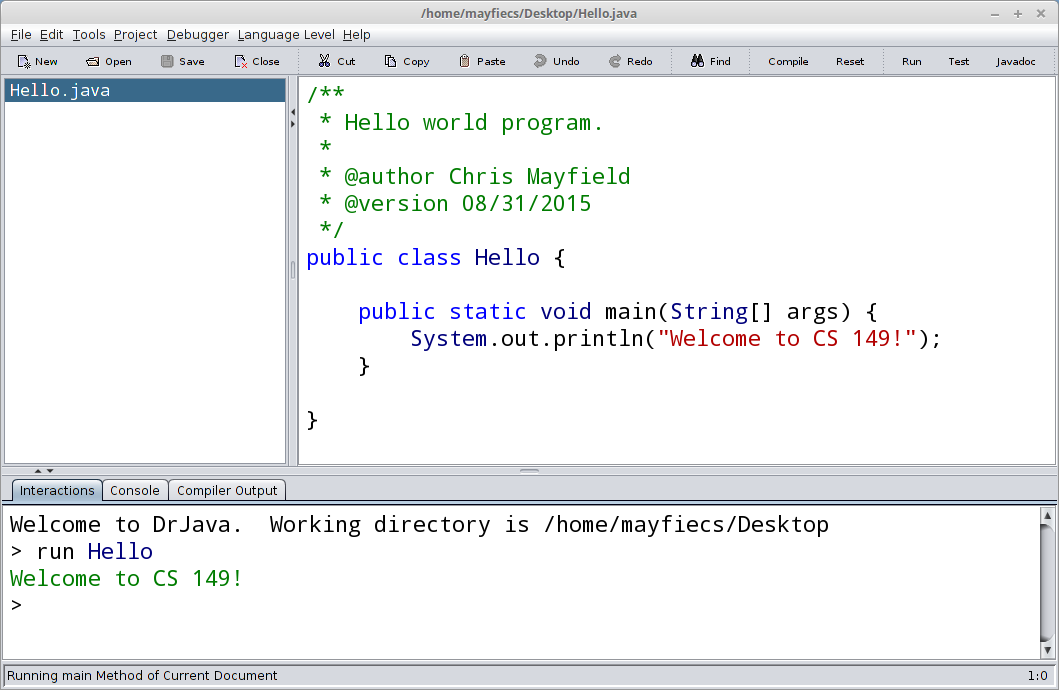
\includegraphics[height=3.65in]{hello1.png}
\end{center}


\quest{8 min}


\Q What is the name of the class?
What is the name of the file?
What directory is it in?

\begin{answer}
Class name: \texttt{Hello} ~~~
File name: \texttt{Hello.java} ~~~
Directory: \texttt{/home/mayfiecs/Desktop}
\end{answer}


\Q How many lines of code is the above program?
How many statements does it have?

\begin{answer}
The source file has 13 lines.
There is only one statement (the \java{println}).
\end{answer}


\Q What is the purpose of the first six lines?
What is the purpose of the two blank lines?

\begin{answer}
The first six lines describe what the program does and who wrote it.
The last six lines define the \java{Hello} class.
When you run \java{Hello}, it prints a welcome message.
\end{answer}


\Q Describe in your own words what \java{System.out.println} means.
Be very specific.

\begin{answer}
The \java{println} method displays a message on the screen, followed by a newline character.
\end{answer}
